\section{Question MLN1}


\subsection{Question}
Using the small Wikipedia example, choose 10 words and create stem classes as per the algorithm on pp. 191-192.

\begin{enumerate}
    \item For all pairs of words in the stem classes, count how often they co-occur in text windows of W words. W is typically in the range 50-100.
    \item Compute a co-occurrence or association metric for each pair. This measures how strong the association is between the words.
    \item Construct a graph where the vertices represent words and the edges are between words whose co-occurrence metric is above a threshold T .
    \item Find the connected components of this graph. These are the new stem classes.
\end{enumerate}


\subsection{Approach}
The following were selected as the words to be stemmed using the approach outlined on pp. 191-192 of the textbook:

\begin{itemize}
    \item affiliates
    \item affiliation
    \item affiliated
    \item fire
    \item firing
    \item fired
    \item changing
    \item changed
    \item changes
    \item change
\end{itemize}

The python scripts \texttt{stem.py} and \texttt{mln1.py} were written to complete this task and can be found in Listings \ref{listing:stem} and \ref{listing:mln1}, respectively.  After performing initial stemming using nltk's SnowballStemmer \cite{py:nltk}, Dice's coefficient was used as a measure of word co-occurrence with a window size of the entire document.  A threshold of 0.1 was used to determine which pairs of words should have edges in the resulting word co-occurrence graph.  


\subsection{Results}
The NetworkX library \cite{py:nx} was used to construct the graph found in Figure \ref{fig:graph} and to find the connected components.\\


\begin{figure}[h!]
\centering
\label{fig:graph}
\fbox{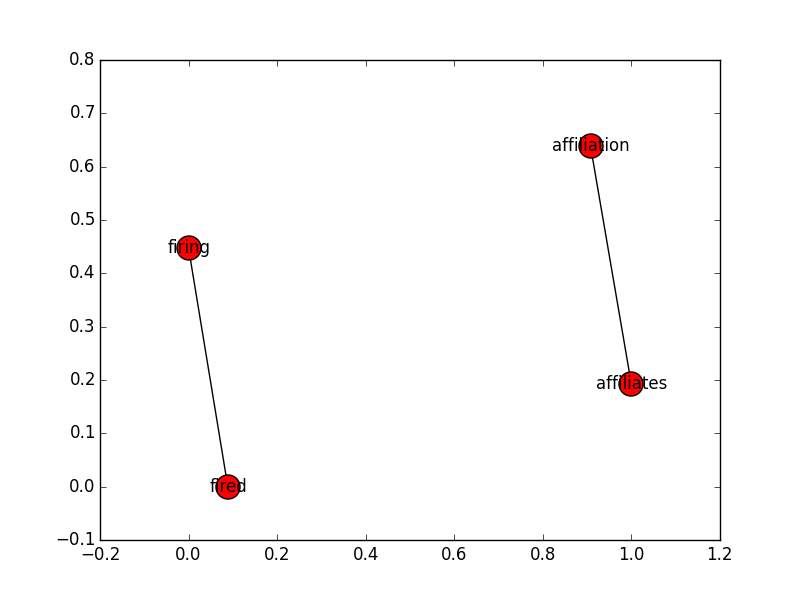
\includegraphics[scale=.6]{code/figure1.png}}
\caption{Graph Visualization of Stem Clusters}
\end{figure}


The initial stem classes after applying the Dice's coefficient threshold of 0.1:\\

\noindent
fire: fire, firing, fired\\
affili: affiliation, affiliates, affiliated\\
chang: changing, changed, changes, change\\


The final connected components from the resulting graph:\\

\noindent
fire: firing, fired\\
affili: affiliation, affiliates\\
